\section{Results}
\label{sec:results}

In this section we demonstrate the efficacy and tractability of our novel framework by calculating the first known optimal solutions to three difficult nonlinear sequential decision problems. We note that while dOp~\cite{Gao2013} offers strong {\footnotesize $ \delta $}-optimality guarantees, we found that nonlinear solvers such as $ \mathtt{fmincon} $~\cite{MATLAB_2010} perform comparably well at optimization and are much more efficient, hence we use $ \mathtt{fmincon} $.

{\centering
    \begin{figure}[ht]
        \begin{tabular}{cc}
            \begin{subfigure}{0.24\textwidth}\centering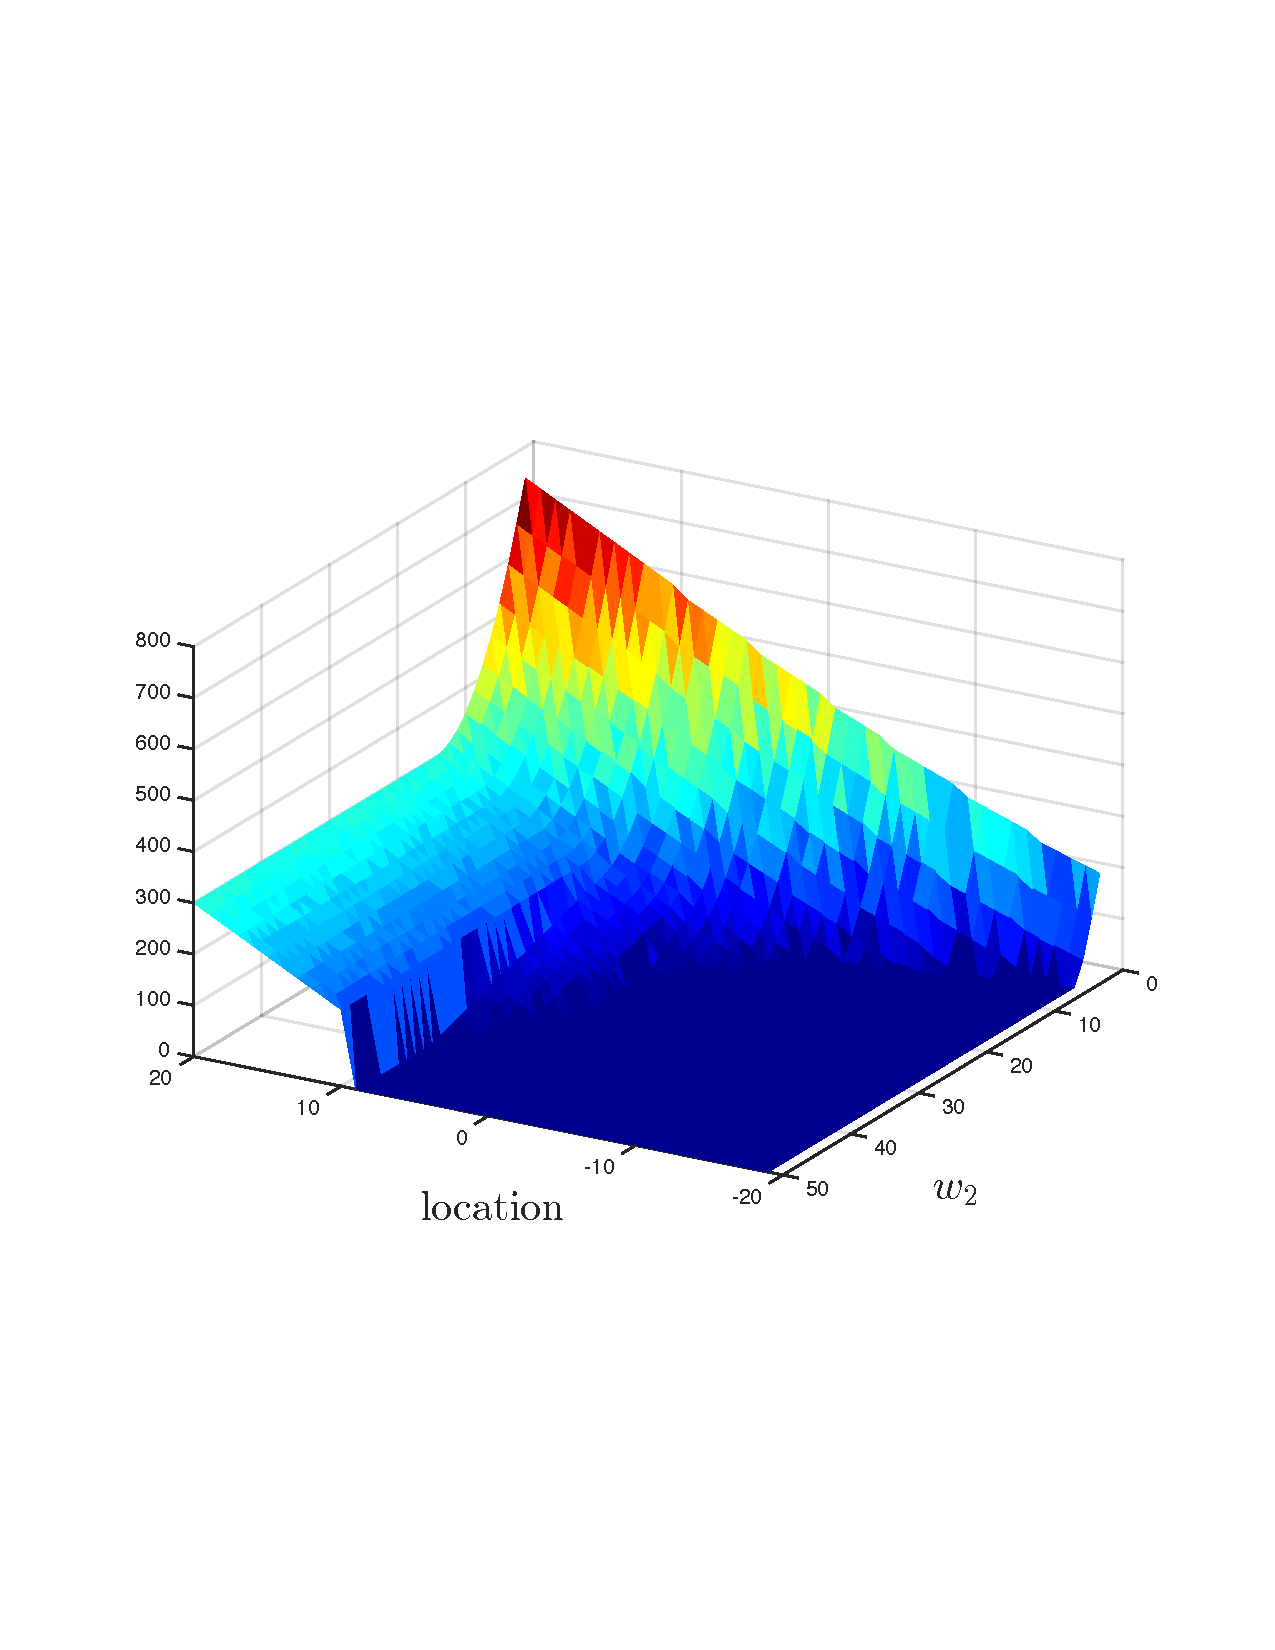
\includegraphics[width=\textwidth]{images/robot_vf_new}\caption{{\footnotesize $V^{\pi^{*}}(loc, w_2; w_1 = 1.0)$} }\label{fig:navigation_vf}\end{subfigure}&
            \begin{subfigure}{0.24\textwidth}\centering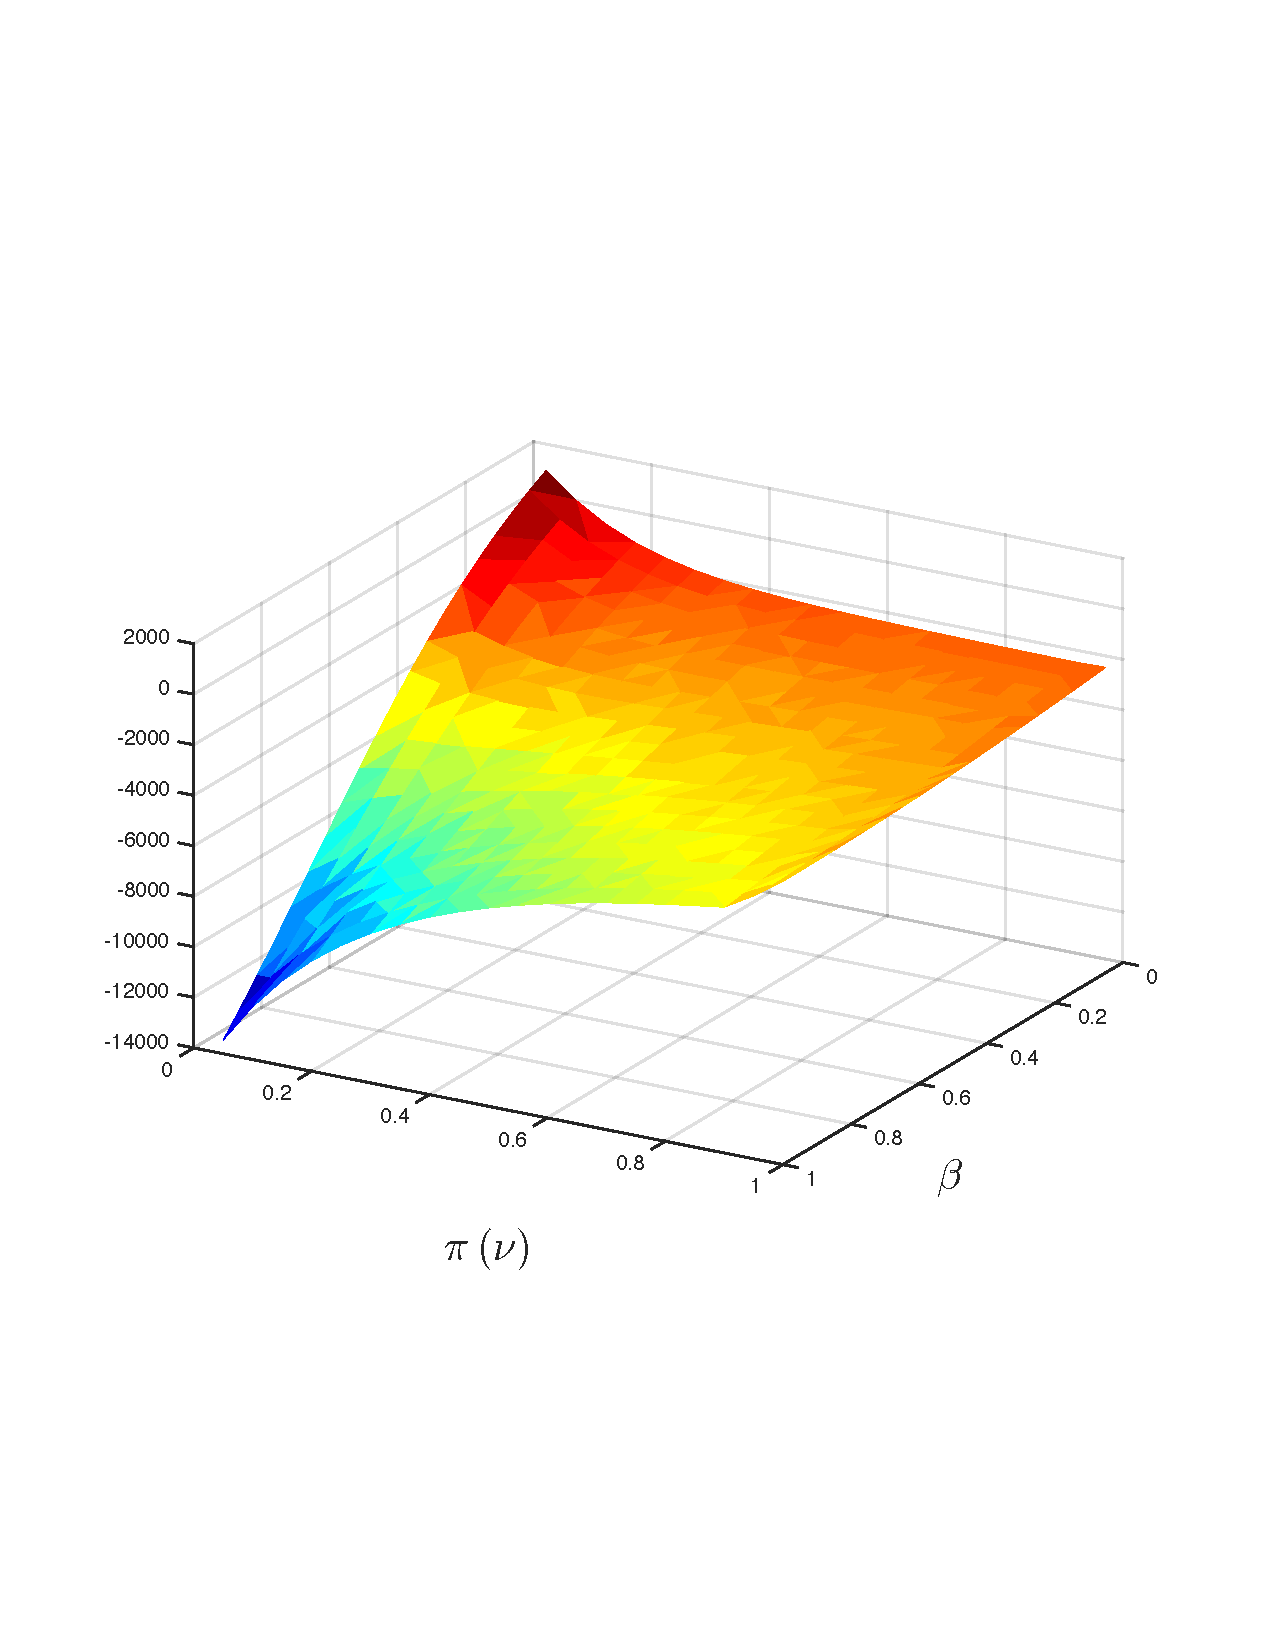
\includegraphics[width=\textwidth]{images/sir_vf_new}\caption{{\footnotesize $V^{\pi^{*}}(\beta, \nu; s, i, r, \lambda, \\\hspace{\textwidth}\qquad cost_{\mathtt{inf}}, cost_{\mathtt{vaccine}})$}}\label{fig:sir_vf}\end{subfigure}
            \\
            \begin{subfigure}{0.24\textwidth}\centering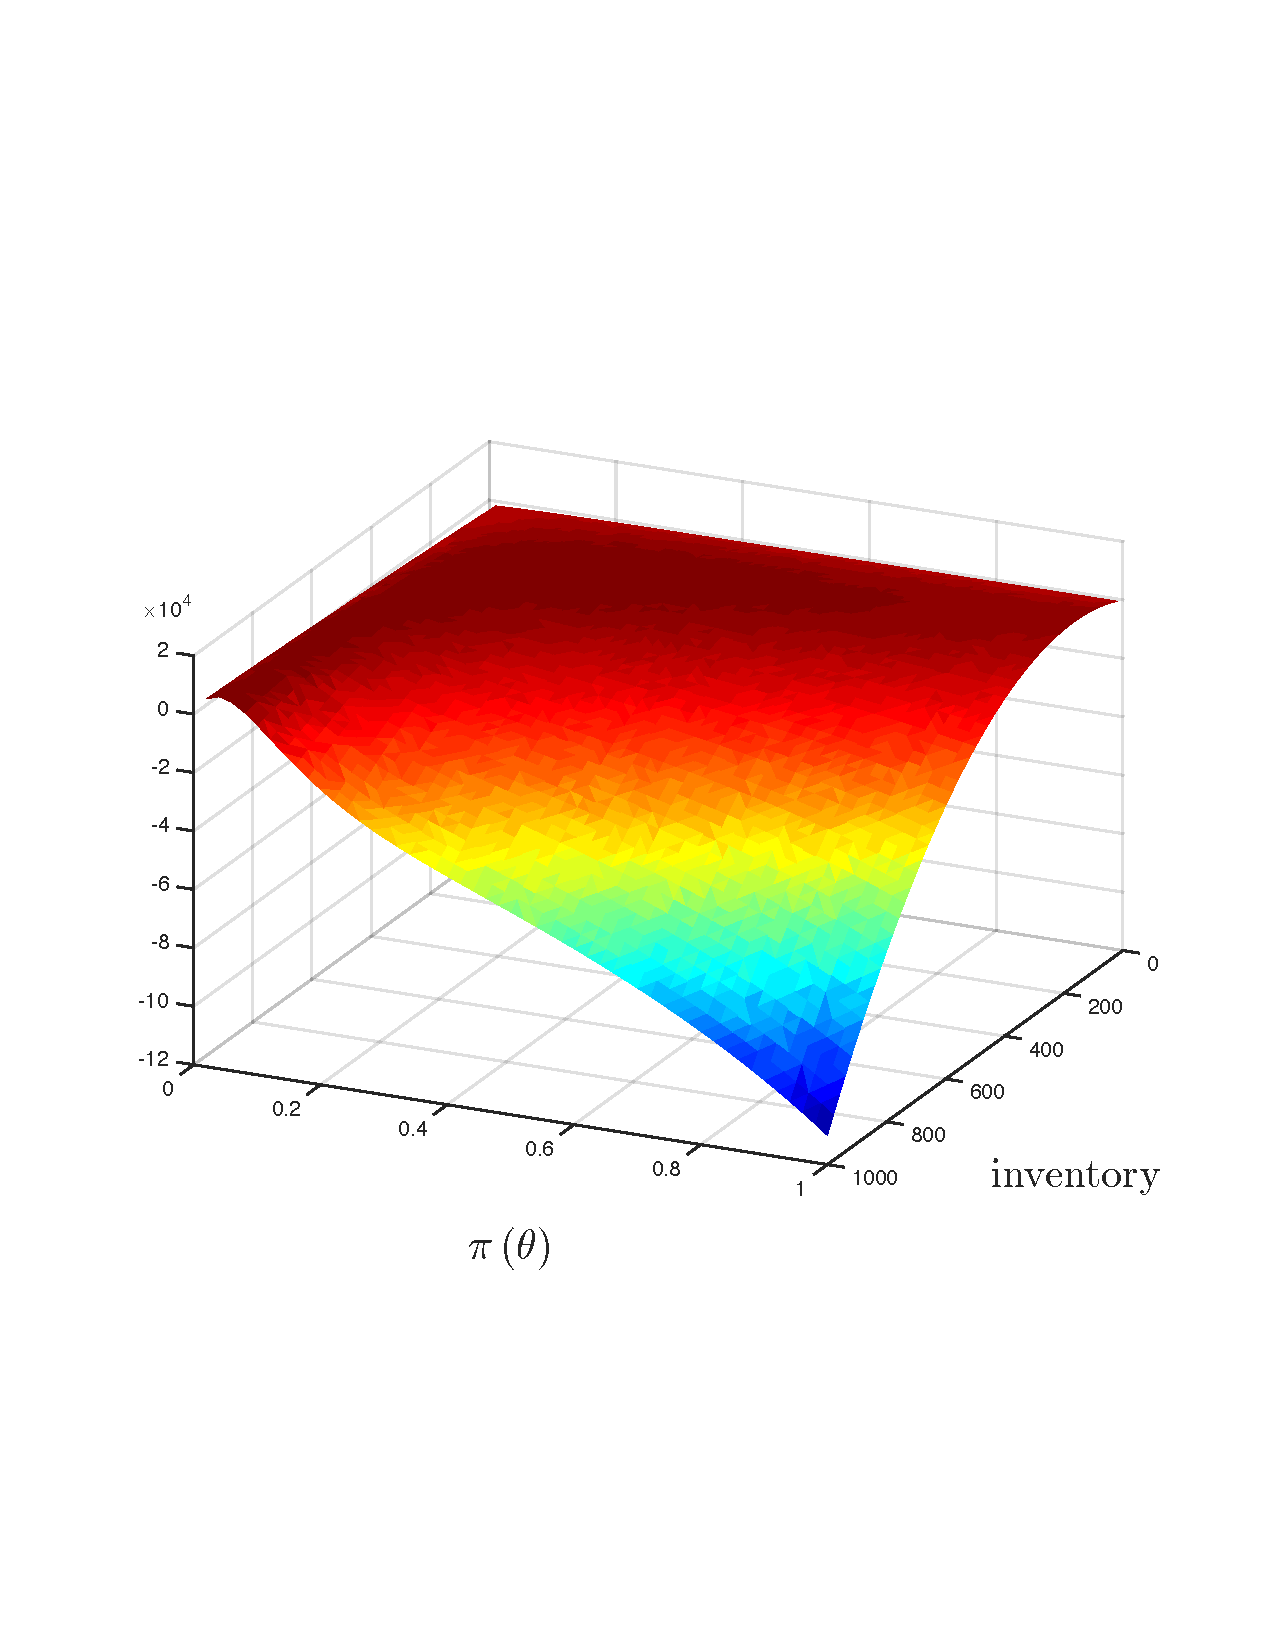
\includegraphics[width=\textwidth]{images/oe_vf_new}\caption{{\footnotesize $V^{\pi^{*}}(\theta, inv; \\\hspace{\textwidth}\qquad p = 55.0, \kappa = 0.165)$}}\label{fig:oe_vf}\end{subfigure}&
            \begin{subfigure}{0.24\textwidth}\centering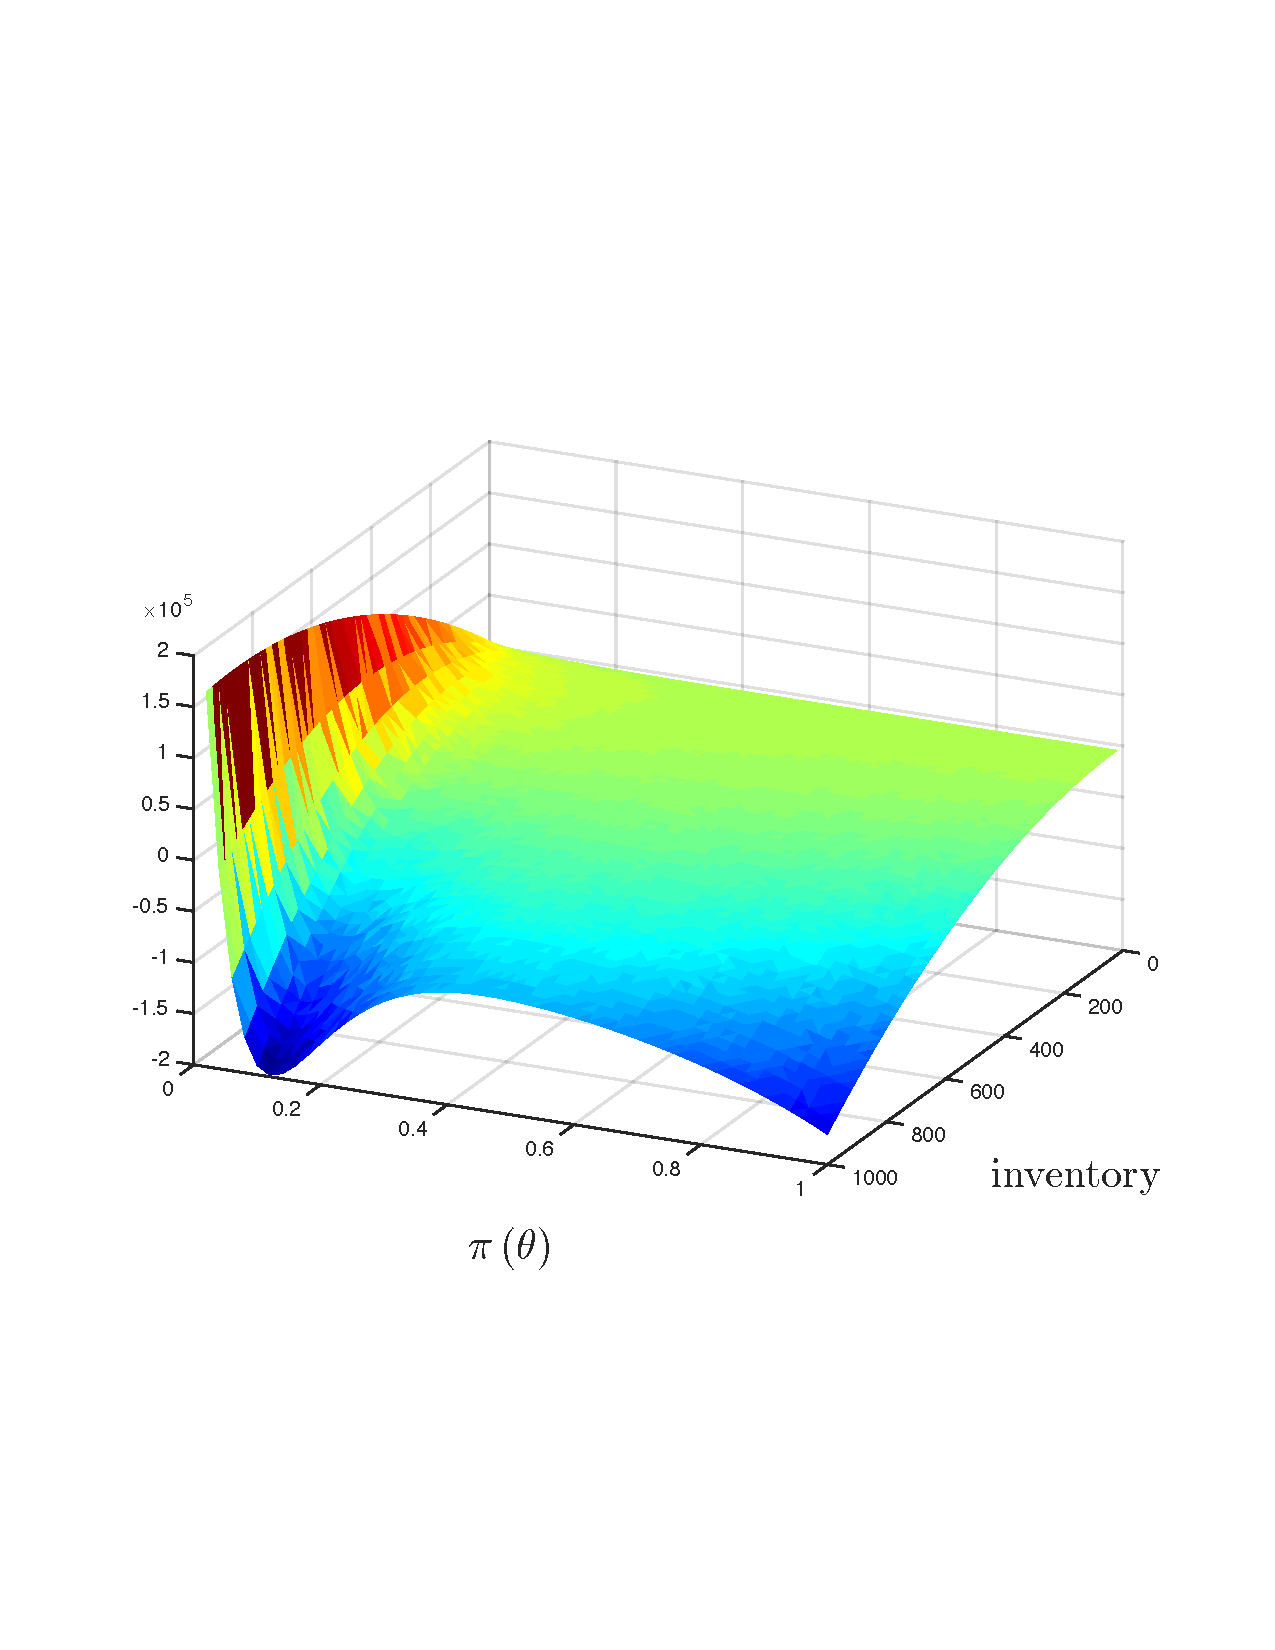
\includegraphics[width=\textwidth]{images/oe_vf_deriv_new}\caption{{\footnotesize $\nabla_{\theta} V^{\pi^{*}} (\theta, inv; \\\hspace{\textwidth}\qquad p = 55.0, \kappa = 0.165)    $}}\label{fig:oe_vf_deriv}\end{subfigure}\\            
        \end{tabular}
        \caption{Optimal Value functions for each domain.}        
        \label{tab:vf_Results}
        \vspace{-3mm}
    \end{figure}
}

{\centering
    \begin{figure}[ht]
        \begin{tabular}{cc}
            \begin{subfigure}{0.2\textwidth}\centering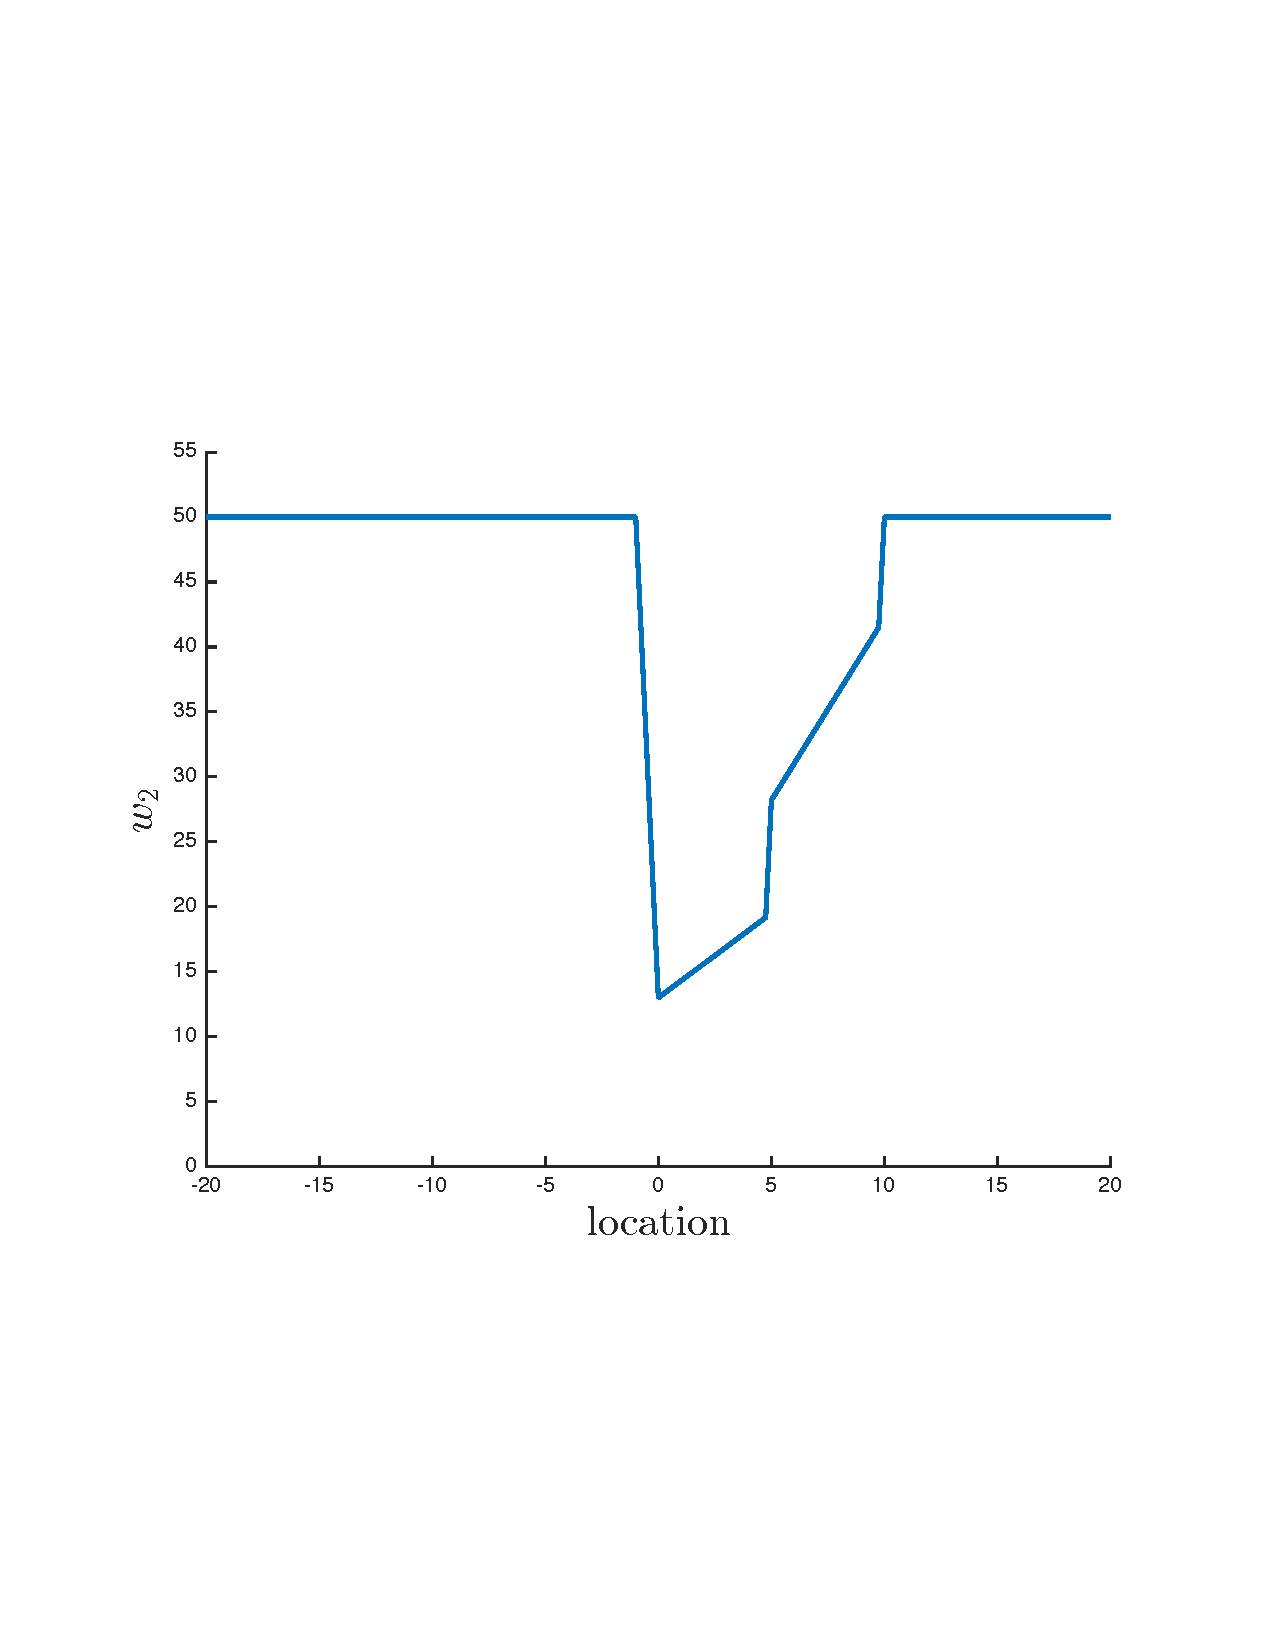
\includegraphics[width=\textwidth]{images/robot_opt_new}\caption{Max {\footnotesize $w_2 \in \left[0.0, 50.0 \right]$} for $ \tilde{\pi} $}\label{fig:navigation_opt}\end{subfigure}&            
            \begin{subfigure}{0.2\textwidth}\centering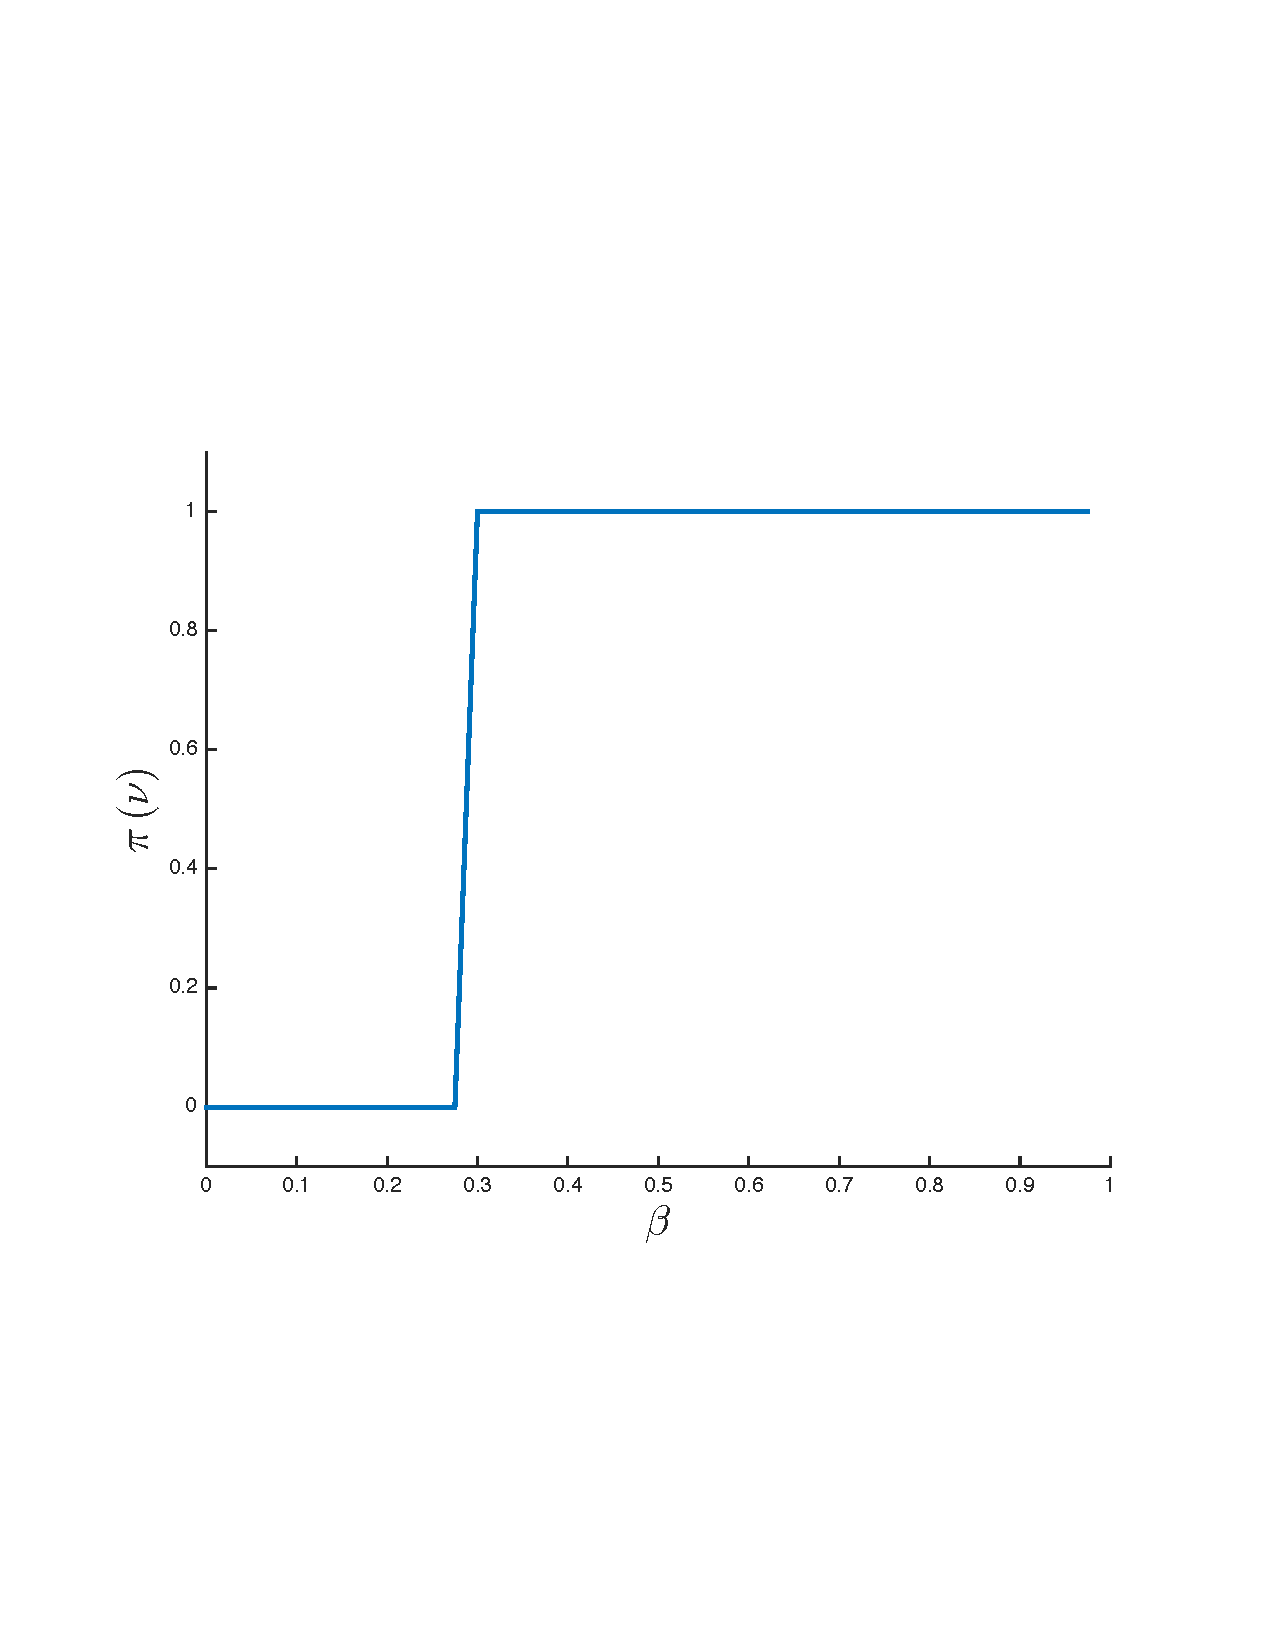
\includegraphics[width=\textwidth]{images/sir_opt_new}\caption{Optimal {\footnotesize $ \nu $} for {\footnotesize $ \beta \in \left[ 0.0, 1.0 \right] $}}\label{fig:sir_opt}\end{subfigure}
            \\
            \begin{subfigure}{0.2\textwidth}\centering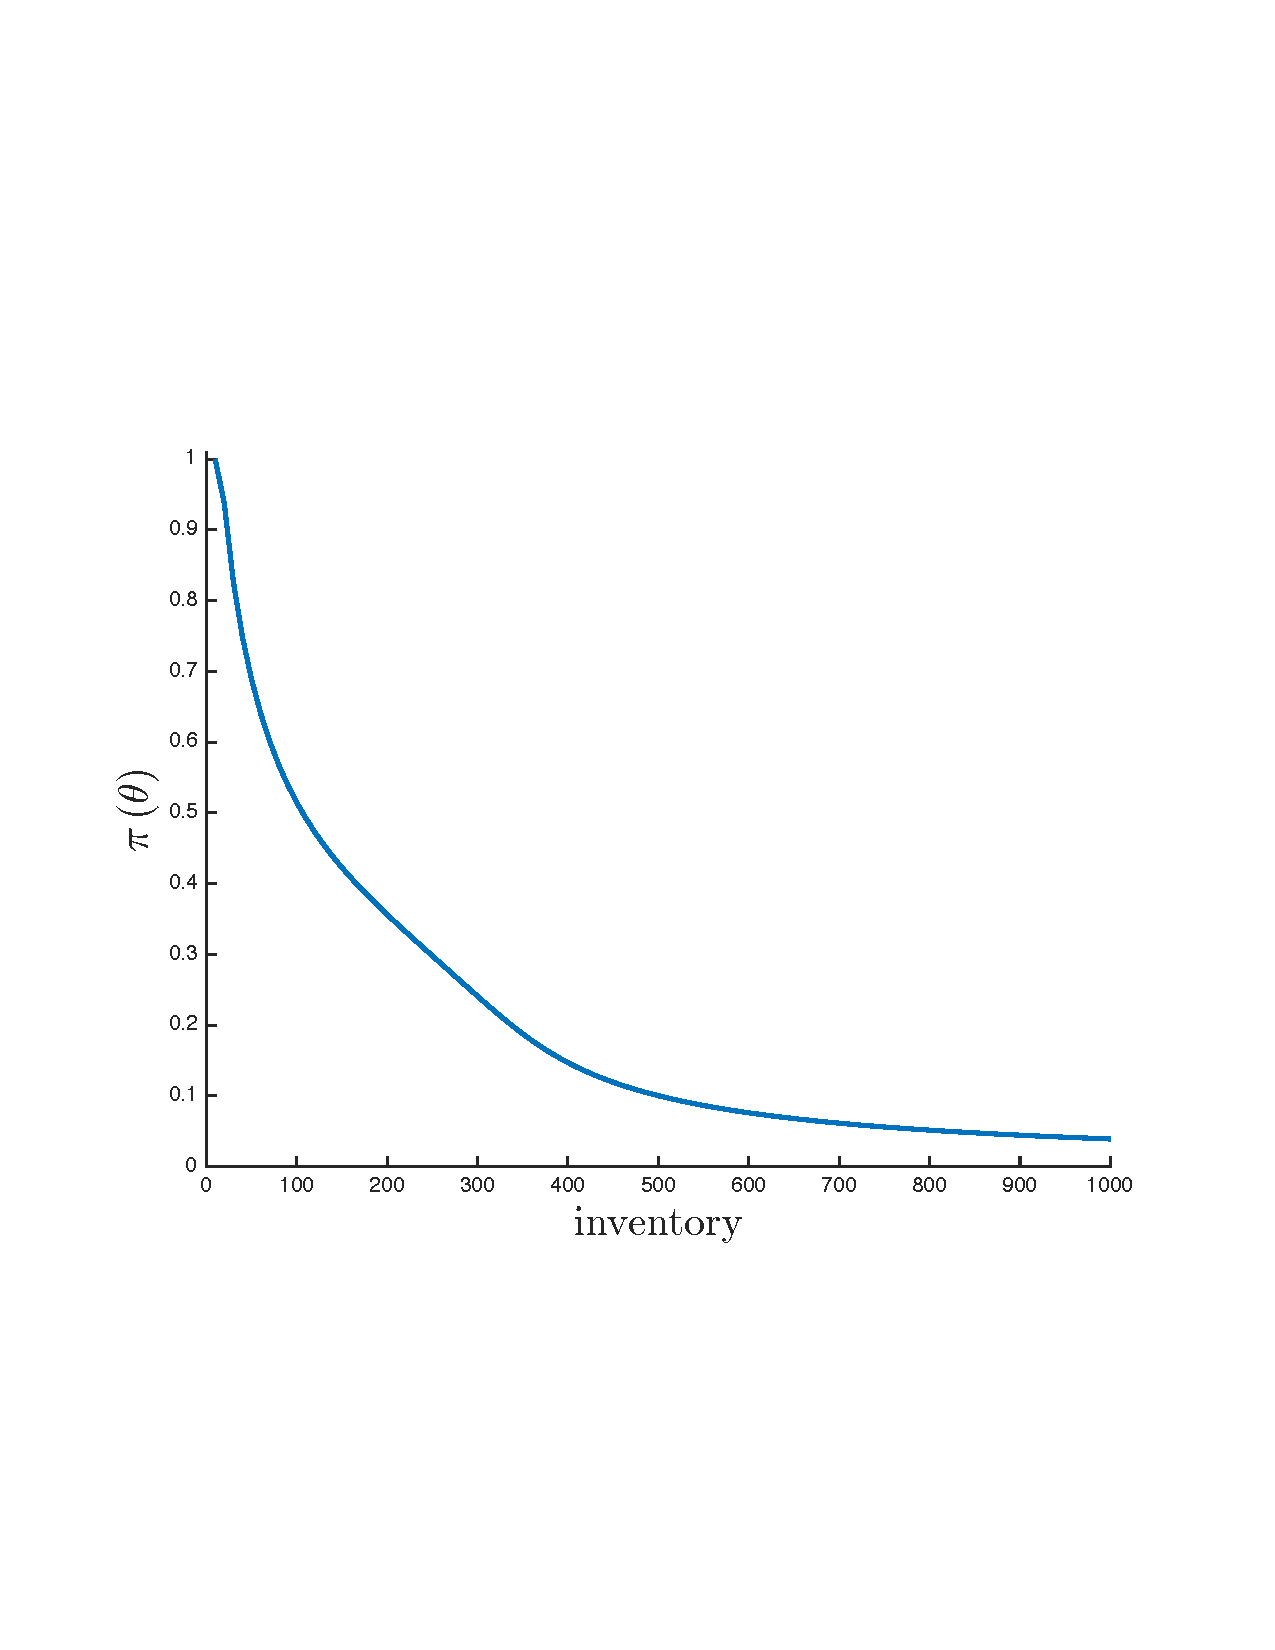
\includegraphics[width=\textwidth]{images/oe_opt_new}\caption{Optimal {\footnotesize $ \theta $} for {\footnotesize $ inv \in \left(0.0, 1000.0 \right) $}}\label{fig:oe_opt}\end{subfigure}&
            \\
        \end{tabular}
        \caption{Nonlinear optimization for each domain.}        
        \label{tab:opt_results}
        \vspace{-3mm}
    \end{figure}
}

\subsection{Inverse Learning for Multi-objective Navigation}
\label{sec:results_navigation}

%In this domain we consider an autonomous vehicle moving in one dimension towards a goal region. At each stage the vehicle faces a trade-off between reaching the goal region and incurring a movement cost. 
The domain is specified as follows: {\footnotesize $ \State = \left\langle loc \right\rangle$}, where $ loc $ is the location of the vehicle. {\footnotesize $ \Action \in \left\lbrace 0.0, 5.0 \right\rbrace $} is the amount by which vehicle moves relative to its current location. {\footnotesize $ \Transition\left( loc' | loc, a \right) = \delta \left[ loc' + (loc + a) \right] $}, where {\footnotesize $ a \in \Action $}. {\footnotesize $ \Reward\left(\vec{w}, loc, loc'\right) = w_1 \cdot \Reward_{\mathtt{region}} + w_2 \cdot \Reward_{\mathtt{move}} $} where,

{\footnotesize 
    \abovedisplayskip=10pt
    \belowdisplayskip=0pt
    \renewcommand{\arraystretch}{1.5}
    \begin{tabular}{ll}    
        $ \Reward_{\mathtt{region}}(loc') = $ &  $ \Reward_{\mathtt{move}}(loc, loc') =  $ \\
        \qquad $ \begin{cases}
        (loc' \leq 10.0 ) : 				& loc' \\
        \text{otherwise} : 					& 0.0 \\
        \end{cases} $ 						& \qquad $ - (loc' - loc)  $\\
%        $ \Reward_{\mathtt{move}}(loc, loc') = - (loc' - loc)$ & $ $ \\                        
    \end{tabular}
} 

At each stage the vehicle faces a trade-off between reaching the goal region and incurring a movement cost. Figure~\ref{fig:navigation_vf}, which shows the optimal value function at {\footnotesize$ \Horizon = 15 $}, 
reveals that the vehicle is willing to incur a cost that is inversely proportional to its distance from the goal region. In Figure~\ref{fig:navigation_opt} we utilise techniques from inverse reinforcement learning~\cite{Ng_ICML_2000} to learn the parameters (weights) of the multi-objective reward under the following sub-optimal policy: {\footnotesize $ \tilde{\pi}(0 < loc < 10) = 5.0,  \tilde{\pi}(loc < 0 \,\mathrm{or}\, loc > 10) = 0.0$}. We observe that when {\footnotesize $a = 0.0$}, {\footnotesize $ w_2 $} is at its maximum allowable value and when {\footnotesize $a = 5.0$}, {\footnotesize $ w_2 $} is inversely proportional to the distance from the goal region and movement size.
%As per the Figure~\ref{fig:navigation_vf}, the vehicle is willing to incur a higher {\footnotesize $ w_2 $} the closer it is to the goal region.

\subsection{Influenza Public Health Policy}
\label{sec:results_influenza}

%In this domain we address the optimization of a static parameterized vaccination policy under a model of Influenza epidemiology where the decision maker must balance the cost of vaccination and the burden of disease.
% on the population. 
The domain is specified as follows: {\footnotesize $ \State = \left\langle s, i, r \right\rangle$}, where $ s $, $ i $, and $ r $ refer to the size of the susceptible, infected and recovered sub-populations, respectively. {\footnotesize $ \Action \in \left\lbrace \pi(\nu) \right\rbrace $} where {\footnotesize $\nu \in \left[0.0, 1.0\right]$} is the proportion of $ s $ to vaccinate at each stage. The transition function {\footnotesize \Transition} for each state variable in {\footnotesize \State} is given by:
    {\footnotesize 
        \abovedisplayskip=5pt
        \belowdisplayskip=0pt
        \renewcommand{\arraystretch}{1.5}
        \begin{tabular}{ll}
            $ \Transition\left( s' | s, i, r, \pi(\nu) \right) =$ & $ \delta \left[ s' - (s - \beta \cdot s \cdot i - \pi(\nu) \cdot s) \right] $ \\
            $ \Transition\left( i' | s, i, r, \pi(\nu) \right) =$ & $ \delta \left[ i' - (i + \beta \cdot s \cdot i - \lambda \cdot i) \right] $ \\
            $ \Transition\left( r' | s, i, r, \pi(\nu) \right) =$ & $ \delta \left[ r' - (r + \lambda \cdot i + \pi(\nu) \cdot s) \right] $ \\            
        \end{tabular}
    }%
where {\footnotesize $ \beta $} is the infection rate and {\footnotesize $\lambda$} is the spontaneous recovery rate. The reward is specified as {\footnotesize $ \Reward\left(cost_{\mathtt{inf}}, cost_{\mathtt{vaccine}}, s, i, r, \pi(\nu) \right) = (s \cdot (-cost_{\mathtt{vaccine}} \cdot \pi(\nu) + (1 - \pi(\nu)))) - cost_{\mathtt{inf}} \cdot i + r$}. {\footnotesize $ cost_{\mathtt{inf}} $} is the incident cost of infection
%, akin to a burden of disease, 
and {\footnotesize $ cost_{\mathtt{vaccine}} $} is the unit cost of vaccination. We assume that the total population is constant and that vaccinated individuals go straight from {\footnotesize $ s $} to {\footnotesize $ r $} without being infected. The decision maker must balance the cost of vaccination and the burden of disease.
on the population. 

Figure~\ref{fig:sir_vf} shows the optimal value function at {\footnotesize$ \Horizon = 7 $} when {\footnotesize $ s = 1000.0, i = 100.0, r = 0.0, \lambda = 0.25 $}, {\footnotesize $ cost_{\mathtt{vaccine}} = 4.0$} and {\footnotesize $ cost_{\mathtt{inf}} = 10.0 $}. The value function shows that it is not always optimal to vaccinate the entire population. In fact, 
%the non-convex optimization of the value function with respect to the policy parameter {\footnotesize $ \nu $}, shown in 
Figure~\ref{fig:sir_opt} reveals that vaccinating the entire population 
is only optimal when {\footnotesize $ \beta > 0.25 $}, that is, when the \textit{basic reproductive ratio} {\footnotesize $ R_0 \,(= \beta/\lambda)$}~\cite{Heffernan_2005} exceeds 1.0. 
%is optimal to vaccinate the entire population only when the infection rate {\footnotesize $ \beta > 0.25 $}. When  {\footnotesize $ \beta > 0.25 $}, the \textit{basic reproductive ratio} {\footnotesize $ R_0 \,(= \beta/\lambda)$}~\cite{Heffernan_2005} exceeds 1.0. 
%{\footnotesize $ R_0$} indicates the average number of secondary cases produced by an infected individual in a completely susceptible population and scenarios where {\footnotesize $R_0 > 1.0$} can lead to an epidemic. 
Scenarios where {\footnotesize $R_0 > 1.0$} can lead to an epidemic. 
%The non-convex optimization shows that in this scenario it is worth incurring the vaccination cost to mitigate the costs associated with the burden of disease in an epidemic. 

\subsection{Optimal Execution}
\label{sec:results_oe}

%In this domain we examine the sensitivity of an optimal portfolio transaction model to its parameters. Institutional investors often want to transact a number of shares that exceeds available liquidity. In these situations they face a clear trade-off between the market impact of transacting immediately and the volatility of slow execution. 
The domain is specified as follows {\footnotesize $ \State = \left\langle p, inv \right\rangle$}, where $ p $ is the price of the asset and $ inv $ is the inventory remaining. {\footnotesize $ \Action \in \left\lbrace \pi\left( \theta \right) \right\rbrace$}, where {\footnotesize $ \theta \in \left( 0.0, 1.0\right)$} is the proportion of inventory to be sold. The transition function {\footnotesize \Transition} for each state variable in {\footnotesize \State} is given by:
{\footnotesize 
    \abovedisplayskip=5pt
    \belowdisplayskip=0pt
    \renewcommand{\arraystretch}{1.5}
    \begin{tabular}{ll}
        $\Transition\left( p' | p, inv, \pi\left( \theta \right) \right) =$ & $ \delta \left[ p' - (p - \kappa \cdot (inv \cdot \pi\left( \theta \right)) + \epsilon) \right] $ \\
        $\Transition\left( inv' | p, inv, \pi\left( \theta \right) \right) =$ & $\delta \left[ inv' - (inv - inv \cdot \pi\left( \theta \right)) \right] $ \\
    \end{tabular}
}%
where {\footnotesize $ \kappa > 0$} is a market-impact parameter and {\footnotesize $ \epsilon $} is a discrete noise parameter. The reward is specified by {\footnotesize $ \Reward\left(p', inv, \pi\left( \theta \right) \right) = p' \cdot inv \cdot \pi\left( \theta \right)$ }. Institutional investors often want to transact a number of shares that exceeds available liquidity. In these situations they face a clear trade-off between the market impact of transacting immediately and the volatility of slow execution. 

Figures~\ref{fig:oe_vf} and~\ref{fig:oe_vf_deriv} show the optimal value function at {\footnotesize $ \Horizon = 10 $} and its derivative with respect to the parameter {\footnotesize $ \theta$}, respectively. It is evident that the optimal proportion of shares to be sold is inversely proportional to the amount of inventory remaining. When inventory is low, selling a large proportion of shares allows the investor to capture the current price and when inventory is high, selling a lower proportion of shares captures a more stable set of future prices.
%When inventory is low, selling a large proportion of shares allows the investor to capture the current price without having too adverse an effect on future prices. This phenomenon is reversed when inventory is high, with the investor selling a lower proportion of shares to capture a more stable set of future prices by minimising the market impact of their trades. 
This insight is confirmed in Figure~\ref{fig:oe_vf_deriv} which shows that the value function is most sensitive to {\footnotesize $\theta$} when the inventory is high.

\subsection{Time and Space Complexity}

%{\centering
    \begin{figure}[ht]
        \begin{tabular}{cc}
            \begin{subfigure}[b]{0.24\textwidth}\centering 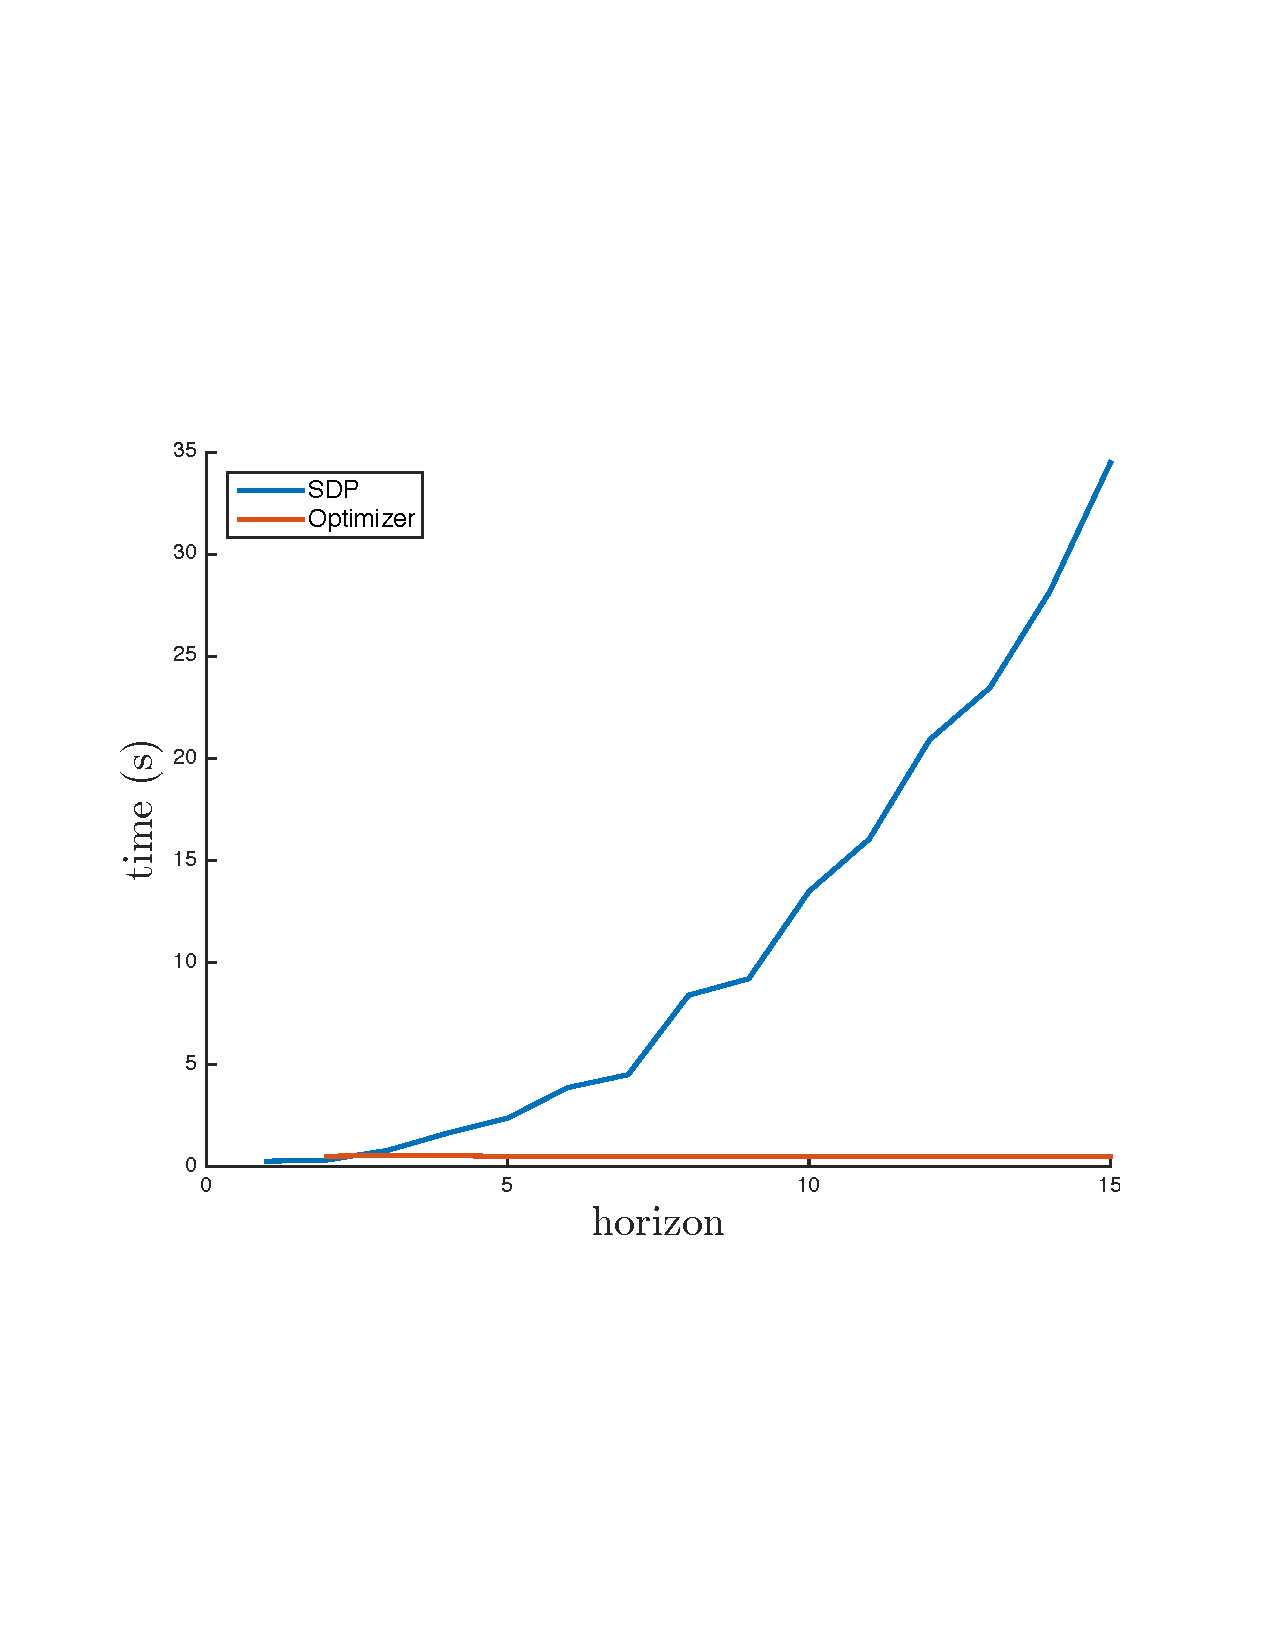
\includegraphics[width=\textwidth]{images/time_plot_new}
                \label{fig:time_complexity}\end{subfigure}\hspace{-1em}
            \begin{subfigure}[b]{0.24\textwidth}\centering 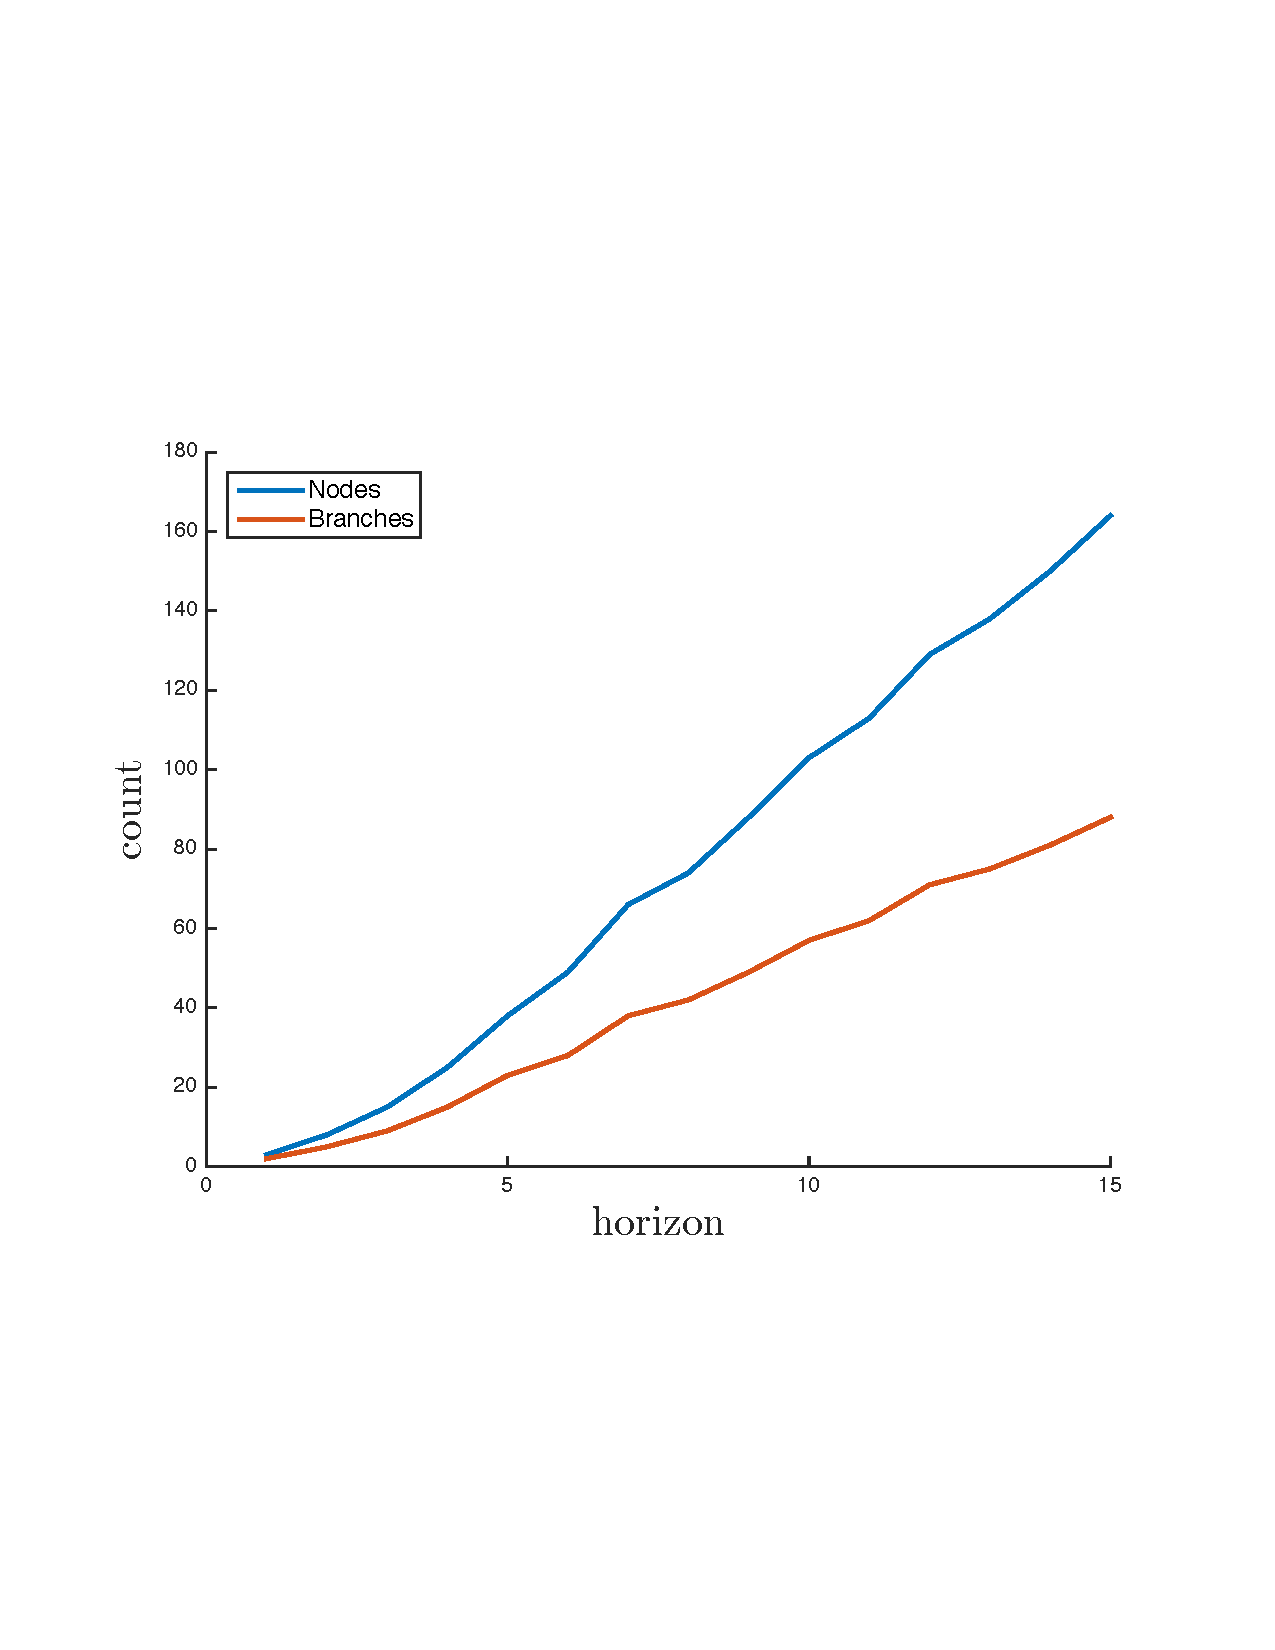
\includegraphics[width=\textwidth]{images/space_plot_new}
                \label{fig:space_complexity}\end{subfigure}
            \\
        \end{tabular}
%        \vspace{-1em}
        \caption{Computational time and space versus {\footnotesize $ \Horizon $} for the multi-objective navigation domain.}
        \label{fig:time_space_complexity}    
        \vspace{-3mm}
    \end{figure}
%}

Figure~\ref{fig:time_space_complexity} shows the relationship between the horizon {\footnotesize $ \Horizon $} and the computational time and space for the largest domain investigated in this section. The computation time and space required to run SDP on PHMDPs increases linearly with the horizon, which is a promising scalability property of the overall framework.